\section{ロボットビューワ}

デフォルトのIrtviewerを作成する(\reffig{irtviewer}).
\begin{verbatim}
(make-irtviewer)
\end{verbatim}
\begin{figure}[htb]
  \begin{center}
    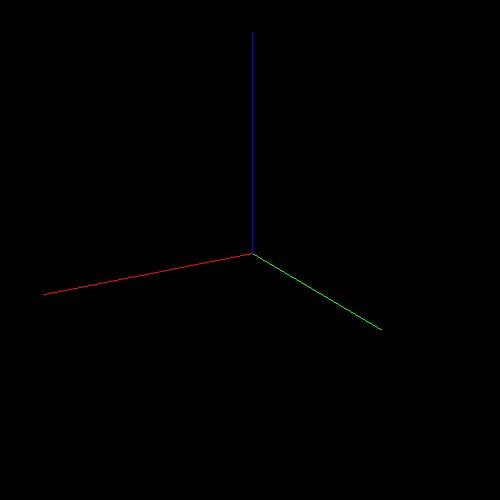
\includegraphics[width=0.50\columnwidth]{fig/irtviewer.jpg}
    \caption{Default irtviewer}
    \labfig{irtviewer}
  \end{center}
\end{figure}

Irtviewerを作成して,xy平面のグリッドを描画する(\reffig{irtviewer-floor}).
\begin{verbatim}
(make-irtviewer)
(send *irtviewer* :draw-floor 100)
(send *irtviewer* :draw-objects)
\end{verbatim}
\begin{figure}[htb]
  \begin{center}
    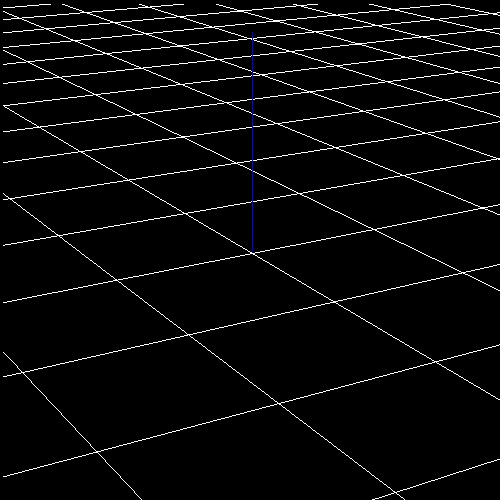
\includegraphics[width=0.50\columnwidth]{fig/irtviewer-floor.jpg}
    \caption{Irtviewer with floor grid}
    \labfig{irtviewer-floor}
  \end{center}
\end{figure}

Irtviewerを作成して,背景を白にして,xy平面のグリッドを黒で描画する(\reffig{irtviewer-floor-white}).
\begin{verbatim}
(make-irtviewer)
(send *irtviewer* :change-background (float-vector 1 1 1))
(send *irtviewer* :draw-floor 100)
(send *irtviewer* :floor-color #f(0 0 0))
(send *irtviewer* :draw-objects)
\end{verbatim}
\begin{figure}[htb]
  \begin{center}
    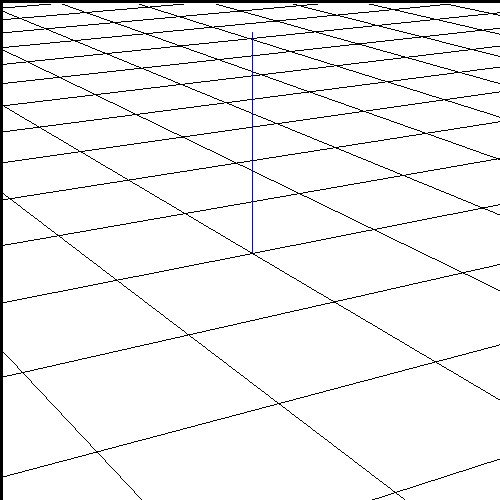
\includegraphics[width=0.50\columnwidth]{fig/irtviewer-floor-white.jpg}
    \caption{Irtviewer with white background and floor grid}
    \labfig{irtviewer-floor-white}
  \end{center}
\end{figure}


\input{irtviewer-func}
